
\section{Introduction}
\label{sec:intro}


The advancements in text-guided image synthesis through diffusion models have garnered considerable attention due to their ability to achieve remarkable realism and diversity \cite{saharia2022imagen,rombach2022latent}. These large-scale models enable image generation from text prompts and have unlocked a new level of creativity. 
As a result, research is intensifying around the applications of these models to manipulate the underlying distributions of images for editing purposes. One striking innovation is the possibility of editing images through intuitive text prompts, giving users the  power to modify images without professional editing skills. {\modified{}This paper focuses} on the prompt-based image editing task as formulated in \cite{mokady2023null}: a user provides an image alongside its textual description. Then, by changing the meaning of the sentence, the user can instruct the model to add, omit, change, or enhance image elements (See Fig.~\ref{fig:teaser} for example). The models implicitly determine which areas of the input image are irrelevant to the target task and should be reconstructed, and which areas require effective modification while preserving the relevant identity and geometry.

The state-of-the-art methods for the prompt-guided editing task require inversion of the target image (see Fig.~\ref{fig:related}). Although inversion processes have greatly improved within Generative Adversarial Networks, they remain a significant hurdle in diffusion models due to their iterative sampling process. Current techniques~\cite{mokady2023null} require repetitive optimization steps, resulting in high computational demands with even moderately-sized images (\(512 \times 512\)), taking upwards of a minute to process per image. Alternatives that reduce computational workload~\cite{mokady2023null,miyake2023negative,parmar2023zero} often compromise on reconstruction quality, resulting in undesired alterations of the input image.


% \setlength{\tabcolsep}{1pt}
  \begin{figure}[t]
    \footnotesize
    \small
    \centering
    \begin{tabular}{m{2.8cm}m{0.5cm}m{2.8cm}}
      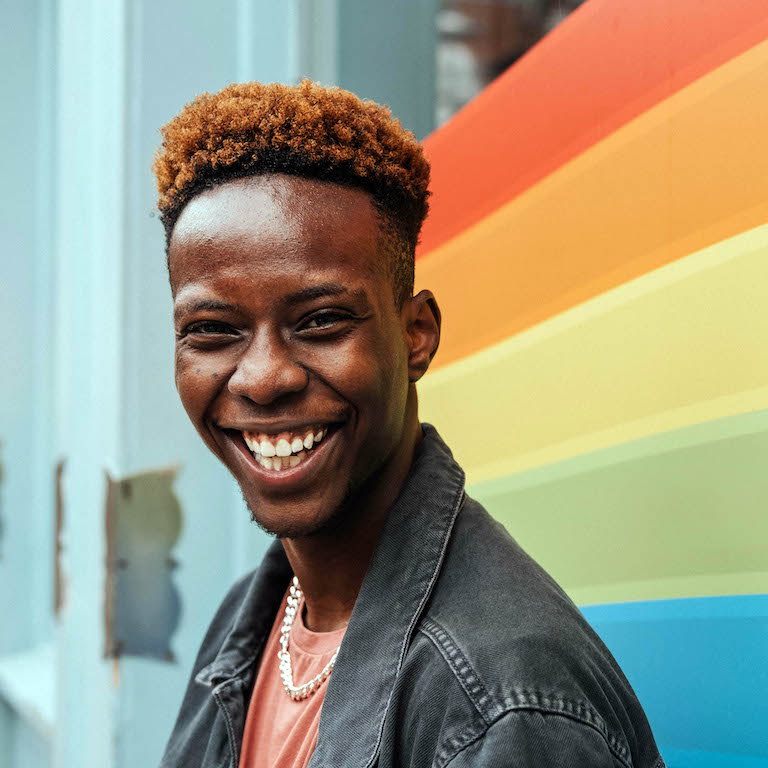
\includegraphics[width=2.8cm, height=2.8cm]{fig/teaser/teaser_1_in.jpg} & $\rightarrow$ & 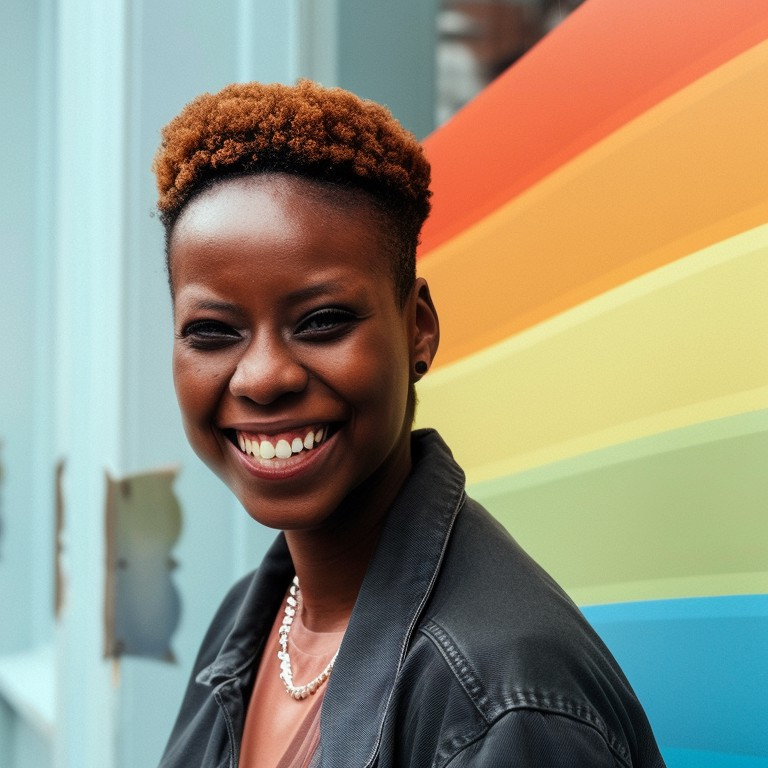
\includegraphics[width=2.8cm, height=2.8cm]{fig/teaser/teaser_1_out} \\
      \multicolumn{3}{c}{``\textit{a \textcolor{BrickRed}{\st{man}} \textcolor{RoyalBlue}{\textbf{woman}} smiling}"} \\
      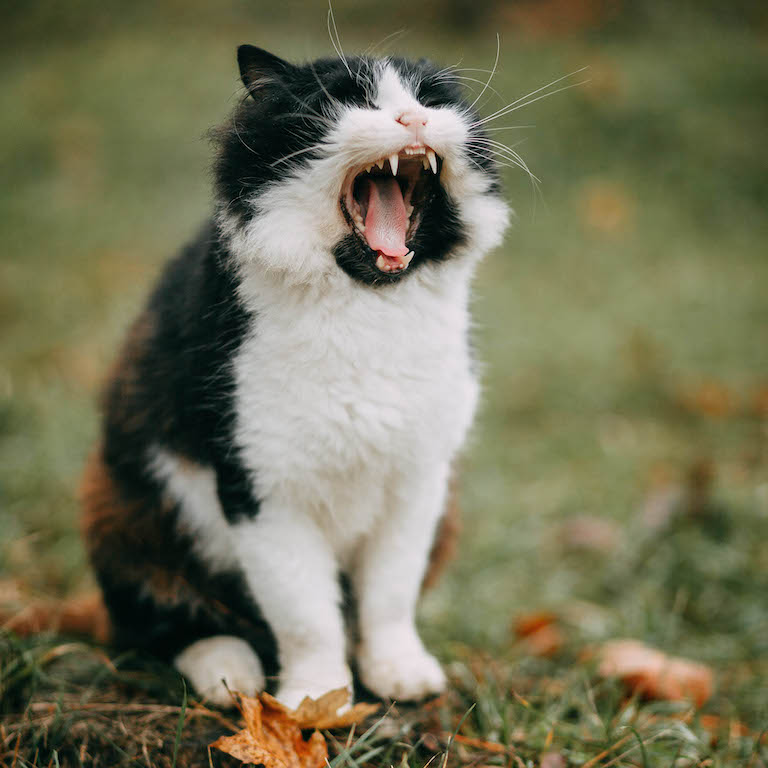
\includegraphics[width=2.8cm, height=2.8cm]{fig/teaser/teaser_2_in.jpg} & $\rightarrow$ & 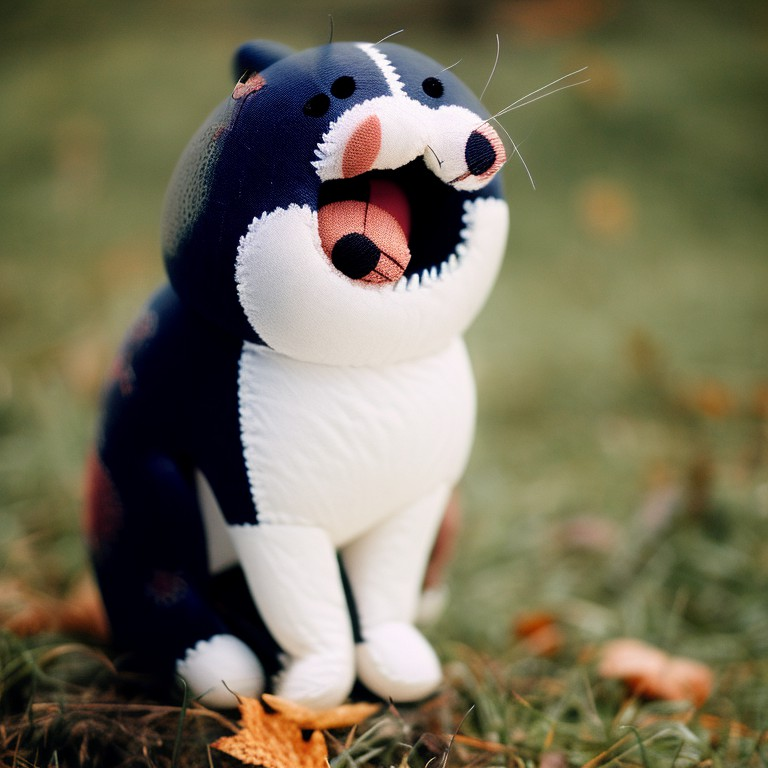
\includegraphics[width=2.8cm, height=2.8cm]{fig/teaser/teaser_2_out} \\
      \multicolumn{3}{c}{``\textit{a \textcolor{RoyalBlue}{\textbf{plush toy}} cat yawning }"} \\
      
    \end{tabular}
    \caption{Prompt-based image editing: the user can add, omit, change, or enhance elements in an image by providing a descriptive prompt of the original image and marking the words that must be removed (in \textcolor{BrickRed}{\textbf{red}}) or added (in \textcolor{RoyalBlue}{\textbf{blue}}).}
    \label{fig:teaser}
  \end{figure}
  

  \begin{figure*}[ht]
    \centering
    % import pdf≤
    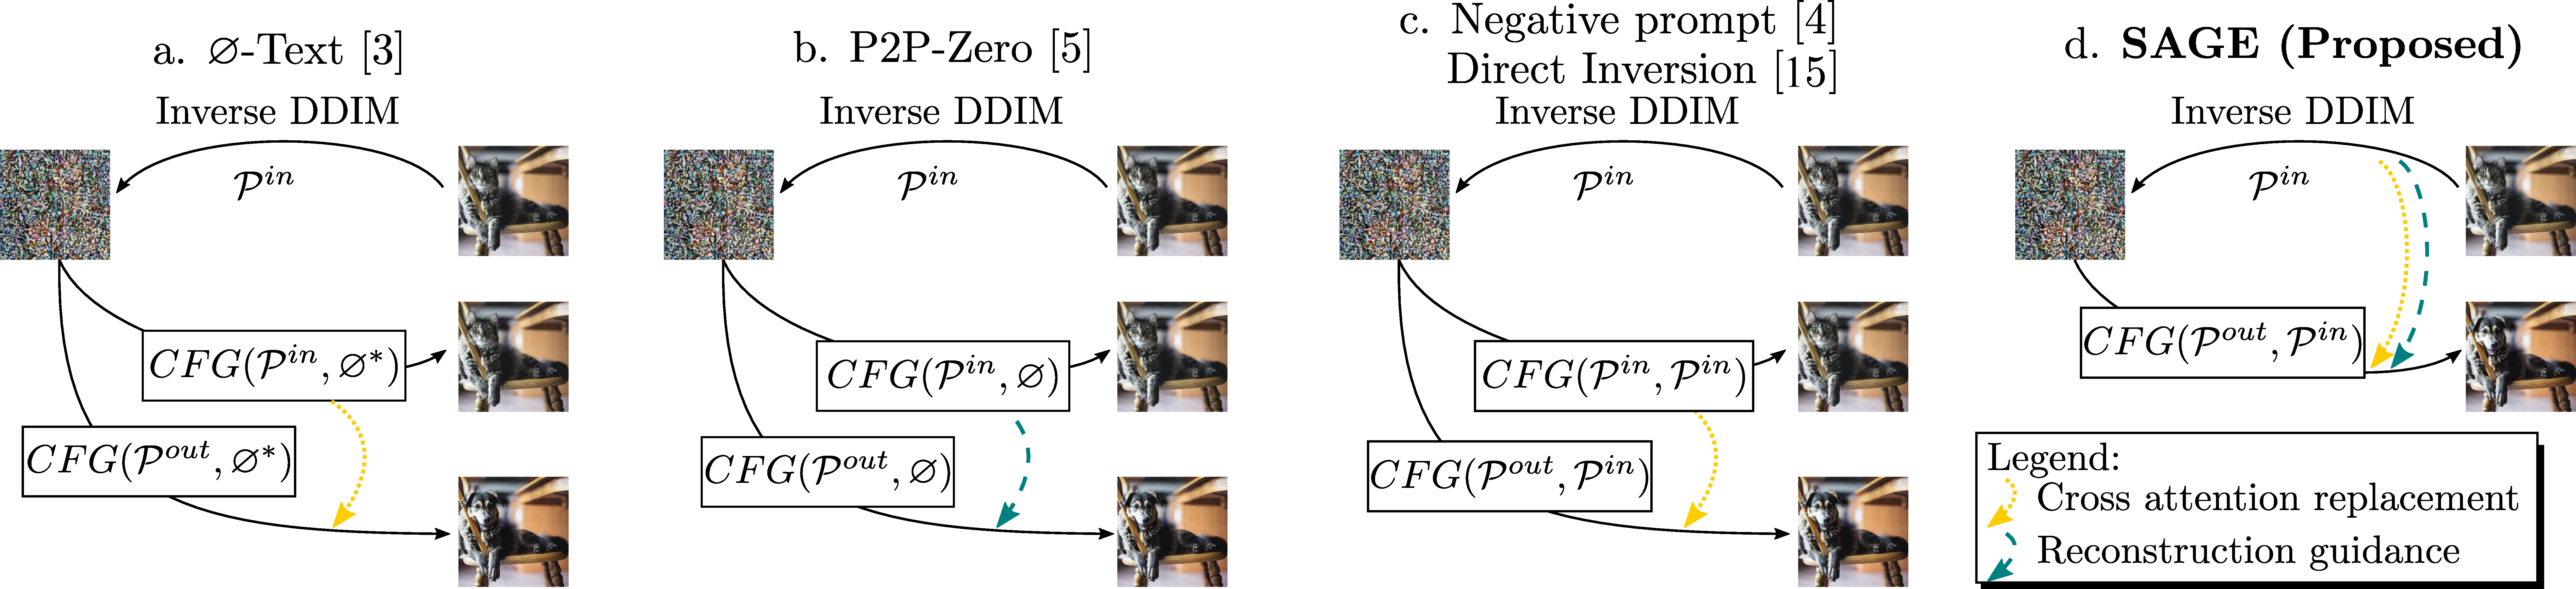
\includegraphics[width=0.9\linewidth]{fig/related.pdf}
    \caption{Comparative Analysis of Diffusion-Based Image Editing Techniques. {\modified{}This review contrasts} existing methodologies, which utilize Classifier-Free Guidance (CFG) \cite{ho2021classifier} with various combinations, including the pretrained null-prompt $\varnothing$, an optimized latent representation $\varnothing^*$, the descriptive prompt of the input image $\pin$, and the target editing prompt $\pout$. 
    }
      \label{fig:related}
    \end{figure*}
  

To address these challenges, {\modified{}this paper introduces} \method{}  (Self-Attention Guidance for Editing), a novel method that reconciles the requirements for computational efficiency and high-fidelity reconstruction, while affording flexible image editing capabilities. Our approach, akin to existing methodologies~\cite{mokady2023null,miyake2023negative,parmar2023zero}, leverages Denoising Diffusion Implicit Model (DDIM) \cite{song2021ddim} inversion. However, it uniquely exploits the intermediate self-attention and cross-attention maps internally computed by the diffusion model during the inverse DDIM process, enabling faithful reconstruction with minimal computational overhead. During the sampling process from random noise to the output image, {\modified{}our method benefits} from a synergistic application of Classifier-Free Guidance (CFG, see Sec~\ref{sec:self_attention_guidance}) alongside a novel reconstruction guidance mechanism based on self-attention reconstruction. This mechanism operates on the self-attention maps within the diffusion U-Net~\cite{ronneberger2015unet}, facilitating a fine trade-off between editing and preservation of the original image details.

In summary, our contribution is threefold:


\begin{itemize}
    \item {\modified{}Introduction of} a novel editing framework utilizing a pre-trained diffusion model that leverages intermediate noise vectors from the inverse DDIM process. This enables the reconstruction to be steered toward the input image, while allowing modifications aligned with textual prompts.
    \item {\modified{}Proposal of} a reconstruction guidance loss term that operates in the self-attention layers of the diffusion network. This term ensures high-fidelity reconstruction in regions unaffected by the editing process without adding major computational overhead.
    \item {\modified{}Experimental validation benchmarks our approach} against recent methods in the field. \method{} outperforms other methods not only in quantitative and qualitative evaluations but also in a comprehensive user study, where it was preferred in over 60\% of cases. Additionally, it ranked first in seven out of 10 quantitative assessments, securing second and third places in the remaining ones.
\end{itemize}



